% Manuscript skeleton — arXiv-ready (pdflatex). Target: <= 15 pages including references.
% Build: cd paper && pdflatex main && bibtex main && pdflatex main && pdflatex main
% Every \todo{} marks a passage the author has to write or decide; every number without
% a \todo is read from the versioned results in ../results/ (state of 2026-09-28).
\documentclass[11pt,a4paper]{article}
\usepackage[margin=2.5cm]{geometry}
\usepackage[utf8]{inputenc}
\usepackage[T1]{fontenc}
\IfFileExists{lmodern.sty}{\usepackage{lmodern}}{}  % Latin Modern when available (arXiv has it)
\usepackage[expansion=false]{microtype}
\usepackage{amsmath,amssymb}
\usepackage{booktabs}
\usepackage{graphicx}
\usepackage{caption}
\usepackage{subcaption}
\usepackage{xcolor}
\usepackage{url}
\usepackage[hidelinks]{hyperref}
\usepackage[numbers,sort&compress]{natbib}
\graphicspath{{figures/}}
\captionsetup{font=small,labelfont=bf}
\newcommand{\todo}[1]{\textcolor{red!70!black}{[\textbf{TODO:} #1]}}
\newcommand{\Rsqm}{R\$/m\textsuperscript{2}}

\title{Location, location, location: does a tabular foundation model need spatial features?\\
\large TabPFN-3.5 against spatial econometrics and gradient boosting on 130{,}000 declared
transaction prices in São Paulo}

\author{Agnaldo Calvi Benvenho\thanks{BP Avaliações e Perícias, Santana do Parnaíba, Brazil;
IBAPE Nacional. \texttt{agnaldo.benvenho@gmail.com}. Code and data:
\url{https://github.com/abenvenho/tabpfn-itbi-sp}.}}
\date{\today\ --- draft}

\begin{document}
\maketitle

\begin{abstract}
Mass appraisal models encode the dependence of property prices on location explicitly, through
spatial weights matrices, spatial lags or engineered neighbourhood features. We ask whether a
tabular foundation model can do without them. TabPFN-3.5 receives the property attributes and the
geographic coordinates as two ordinary numeric columns, with no spatial modelling of any kind, and is
compared with an OLS hedonic model, a spatial autoregressive lag model (SAR, GM estimation) and
XGBoost with a $k$-nearest-neighbour spatial lag, rotated coordinates and nested tuning. The data
are 82{,}187 declared transaction prices from the São Paulo real-estate transfer tax (ITBI) in 2025
and 47{,}810 in the first seven months of 2026, for apartments, houses and commercial units. The
evaluation has two legs: leave-one-block-out cross-validation over ten spatial blocks, and an
out-of-time test that fits on 2025 and predicts 2026. Refutation criteria were fixed in advance:
worse pooled error, losses in most blocks under paired tests, or more residual spatial
autocorrelation (Moran's~$I$) than the explicitly spatial baselines. Out of time, the plain-table
model beats the spatial XGBoost in ten of ten blocks (RMSE $0.265$ vs $0.287$ in log unit price,
MAPE $19.5\%$ vs $21.0\%$, block-bootstrap 95\% CI of the difference $[-0.032,-0.026]$) and leaves
the least residual autocorrelation of the four models ($I = 0.092$). Across unseen blocks it ties
the spatial XGBoost on error but leaves more spatial structure in its residuals ($I = 0.348$ vs
$0.309$), a partial refutation. Permutation SHAP shows the two coordinates as the strongest inputs.
\todo{Sharpen the last sentence and add one on implications for appraisal practice.}
\end{abstract}

\noindent\textbf{Keywords:} mass appraisal; tabular foundation models; TabPFN; spatial
autoregression; spatial cross-validation; hedonic prices; São Paulo.

\section{Introduction}
\label{sec:intro}

\todo{Two to three paragraphs. (1) The problem: mass appraisal at city scale, the role of location,
and the engineering cost of explicit spatial modelling (weights matrices, lags, GWR-style local
models) that must be redone per city and dataset. (2) Tabular foundation models: in-context
learning on synthetic priors \citep{hollmann2023tabpfn,hollmann2025nature,priorlabs2026tabpfn3};
the open question of whether spatial dependence is learned from raw coordinates. (3) Contribution
and the falsificationist framing: a hypothesis stated with pre-registered refutation criteria and a
comparison deliberately asymmetric against it. Cite the reference study on Belo Horizonte listings
\citep{benvenho2026cead} as the origin of the question.}

The hypothesis is stated so that it can fail:

\begin{quote}
A tabular foundation model that receives only the property attributes and the coordinates as two
plain numeric columns --- no spatial weights matrix, no spatial lag, no engineered neighbourhood
features --- predicts spatially correlated prices as well as, or better than, specialised models
that encode spatial dependence explicitly.
\end{quote}

It is refuted if any of the following holds under a shared protocol: worse pooled RMSE or MAPE;
losses in most spatial blocks under paired tests; or more spatial autocorrelation left in its
out-of-fold residuals than the explicitly spatial models leave in theirs.

Contributions. \todo{Bullet or prose: (i) the first comparison of a tabular foundation model with
spatial econometric and spatially augmented tree baselines on real declared prices at city scale;
(ii) a two-leg protocol with spatial block CV and out-of-time testing and pre-registered refutation
criteria; (iii) a public, reproducible pipeline over open municipal data; (iv) the finding itself,
including the partial refutation.}

\section{Related work}
\label{sec:related}

\todo{Compact, one page at most. Three threads: spatial hedonic models and their estimation
\citep{anselin1988,kelejian1998,lesage2009}; machine learning for mass appraisal with spatial
features, geographically weighted approaches and spatial cross-validation
\citep{roberts2017,meyer2022}; tabular foundation models and in-context learning
\citep{hollmann2023tabpfn,hollmann2025nature,priorlabs2026tabpfn3}. Close with the Belo Horizonte
study \citep{benvenho2026cead} and what this paper changes: listings $\to$ declared prices, one
type $\to$ three, 5k $\to$ 82k rows, added out-of-time leg and residual autocorrelation criterion.}

\section{Data}
\label{sec:data}

\subsection{Source and cleaning}

The São Paulo City Hall publishes every paid form of the real-estate transfer tax (ITBI,
\emph{Imposto sobre Transmissão de Bens Imóveis}) with the declared transaction price, the
cadastral key (SQL: sector, block, lot) and the physical attributes of the property from the annual
property-tax register (IPTU): built and lot area, use, construction standard, corrected completion
year. The 2025 workbook holds 230{,}525 forms and the January--July 2026 workbook 135{,}655.
Coordinates come from the centroids of the fiscal-block polygons of the municipal cadastre
(GeoSampa), so all properties in one city block share a location; distance to the nearest subway
or commuter-rail station is computed from the 203 station points of the same portal.

\todo{Summarise the filter chain from \texttt{data/filter\_report.md} in a short table with the
record counts after each step (transfer type, use codes, area and price bounds, duplicates,
georeferencing).} The cleaned bases hold 82{,}187 transactions for 2025 (training) and 47{,}810 for
2026 (test). A stratified sample of 24{,}000 rows of 2025 (12{,}000 apartments, 7{,}000 houses,
5{,}000 commercial units; ``Level A'') is used wherever the slower baselines must run.

\subsection{Under-declaration}

The ITBI tax base is $\max(\text{declared price},\ \text{assessed reference value})$, so a buyer who
under-declares has no incentive to declare below the assessed value: under-declared cash deals bunch
exactly at it. The pipeline detects that bunching and removes cash transactions declared at the
reference value; financed deals are bank-appraised and kept. \todo{Two sentences with the counts and
a pointer to the diagnostic figure in \texttt{data/underdeclaration\_report.md}.} Section
\ref{sec:robust} repeats the whole analysis on financed deals only.

\subsection{Descriptive statistics}

\begin{table}[h]
\centering\small
\caption{The three bases. Unit value = declared price / built area, in \Rsqm.}
\label{tab:data}
\footnotesize
\begin{tabular}{lrrrrrr}
\toprule
Base & Rows & Apartments & Houses & Commercial & Financed & Median unit value \\
\midrule
2025, full (training) & 82{,}187 & 60{,}067 & 15{,}940 & 6{,}180 & 34\% & 4{,}836 \\
2025, Level A (sample) & 24{,}000 & 12{,}000 & 7{,}000 & 5{,}000 & 30\% & 4{,}715 \\
2026, Jan--Jul (test) & 47{,}810 & 35{,}354 & 9{,}429 & 3{,}027 & 42\% & 4{,}970 \\
\bottomrule
\end{tabular}
\end{table}

\todo{Add a map of the 2026 transactions or reuse Figure~\ref{fig:blocks}(a); one paragraph on
the spatial structure of prices (Moran's $I$ of the raw log unit price on the k-NN-8 matrix).}

\section{Methods}
\label{sec:methods}

\subsection{Target and features}

The target is $y = \ln(\text{price}/\text{built area})$. The information set is the same for every
model: built area, lot area, age, finish grade (IPTU standard level, 0--5), distance to the nearest
station, month index, property type, latitude and longitude. The models differ only in what they
are allowed to do with the last two.

\subsection{Models}

\paragraph{OLS hedonic.} Log-linear in the areas and the distance, quadratic in age, dummies for
type, coordinates as covariates.

\paragraph{SAR lag.} $y = \rho W y + X\beta + \varepsilon$ with a row-standardised $k$-nearest-neighbour
weights matrix ($k = 8$) built inside each training fold, estimated by the generalised-moments
procedure of \citet{kelejian1998} as implemented in \texttt{spreg} \citep{rey2010pysal}.
Prediction for held-out rows uses the reduced form with neighbours drawn from the training rows
only. \todo{Confirm the prediction formula used in \texttt{src/model\_sar.py} and state it.}

\paragraph{XGBoost with spatial features.} The hedonic block above plus UTM coordinates rotated by
$30^\circ$, $45^\circ$ and $60^\circ$ and a $k$-NN-8 spatial lag of the target computed inside the
training fold (leave-one-out for training rows). Hyper-parameters are tuned by nested Optuna
(30 trials, TPE), with an inner leave-one-block-out on the training blocks; the outer test block
never touches tuning \citep{chen2016xgboost,akiba2019optuna}. Three seeds. Geographically weighted
XGBoost, used in the reference study, was timed and found infeasible at this scale
(one local model per training row and bandwidth candidate over a dense $n \times n$ distance
matrix); Appendix~\ref{app:gxgb}.

\paragraph{TabPFN-3.5, plain table.} The nine raw columns, categorical type declared as such,
through the hosted model (\texttt{tabpfn-client} 0.6.0, model version 3.5). Zero-shot, and a
thinking-mode variant in which the fit explores configurations by internal validation on the
training fold (RMSE objective, medium and high effort). No spatial information of any kind beyond
the two coordinate columns. Fitting on 24{,}000 rows takes about 9~s; on 82{,}187 rows, 15~s.

\subsection{Evaluation protocol}

\paragraph{Leg 1: spatial block cross-validation.} Ten $k$-means blocks on the Level A coordinates,
each held out in turn \citep{roberts2017,meyer2022}. Every fold-internal quantity (weights matrix,
spatial lag, tuning) is recomputed on the training blocks only.

\paragraph{Leg 2: out-of-time.} One fit on 2025 (Level A, then the full base), predictions for all
47{,}810 transactions of 2026, one to seven months after the training window. Nothing from 2026
touches fitting or tuning. Leakage check: no transaction (key, date, price) appears in both years;
0.6\% of 2026 rows share a cadastral key with Level A.

\paragraph{Metrics and tests.} RMSE, MAE and $R^2$ in log units, MAPE in price units, mean residual
(bias). Residual spatial autocorrelation by Moran's $I$ \citep{moran1950} on a $k$-NN-8 matrix of
the test coordinates. Paired comparisons over the ten blocks: Wilcoxon signed-rank test on the
per-block metric and a block bootstrap (2{,}000 resamples of blocks) for the pooled difference with
a 95\% percentile interval. Where a model is stochastic, three seeds and a 95\% interval over
seeds.

\section{Results}
\label{sec:results}

\subsection{Leg 1: unseen blocks}

\begin{figure}[t]
\centering
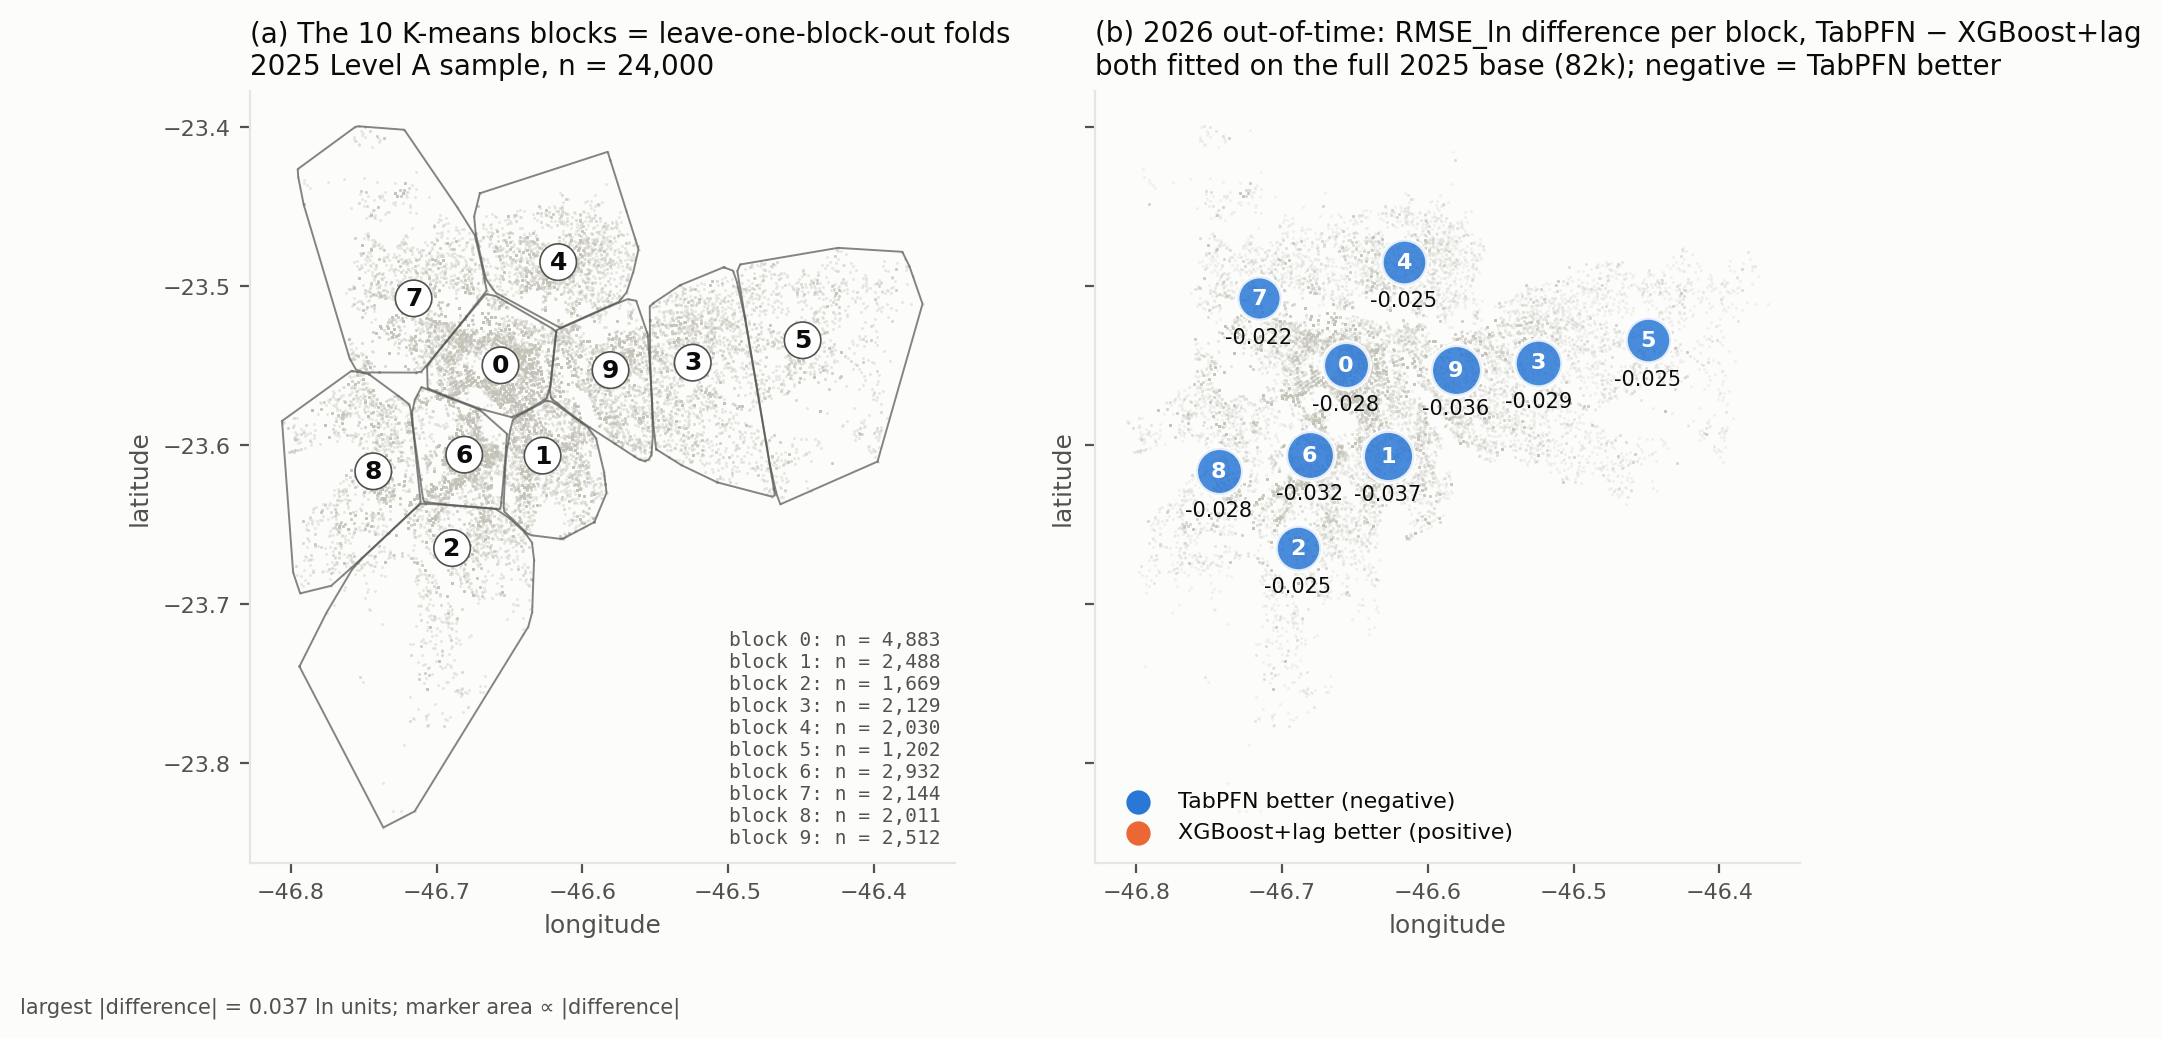
\includegraphics[width=\textwidth]{fig1_blocks_map.png}
\caption{(a) The ten $k$-means blocks of the Level A sample, each held out in turn. (b) Per-block
RMSE difference TabPFN-3.5 $-$ XGBoost+lag on the 2026 test, both fitted on the full 2025 base;
negative in every block.}
\label{fig:blocks}
\end{figure}

\begin{table}[h]
\centering\small
\caption{Leave-one-block-out CV on Level A (24{,}000 rows of 2025). Out-of-fold metrics in log unit
price; Moran's $I$ of the out-of-fold residuals on a $k$-NN-8 matrix. Ranges are over three seeds.}
\label{tab:cv}
\footnotesize
\begin{tabular}{lcccc}
\toprule
Model & RMSE & MAPE & $R^2$ & Moran's $I$ \\
\midrule
Median by type (floor) & 0.497 & 42.1\% & $-0.04$ & 0.446 \\
OLS hedonic & 0.470 & 39.4\% & 0.066 & 0.390 \\
SAR lag, GM ($\hat\rho = 0.91$) & 0.448 & 38.4\% & 0.155 & 0.363 \\
XGBoost, rotated coordinates, no lag & 0.397 & 33.3\% & 0.334 & 0.355 \\
XGBoost, rotated coordinates + $k$-NN-8 lag & \textbf{0.385} (0.384--0.387) & 32.3\% & \textbf{0.376} & \textbf{0.309} \\
TabPFN-3.5, plain table, zero-shot & 0.394 (0.390--0.394) & 32.2\% & 0.346 & 0.348 \\
TabPFN-3.5, plain table, thinking (medium) & 0.389 & \textbf{31.7\%} & 0.362 & 0.342 \\
TabPFN-3.5, plain table, thinking (high) & 0.388 & \textbf{31.7\%} & 0.366 & 0.339 \\
\bottomrule
\end{tabular}
\end{table}

TabPFN-3.5 zero-shot beats the SAR lag model in 8 of 10 blocks ($\Delta$RMSE $= -0.054$, 95\% CI
$[-0.100, -0.014]$, Wilcoxon $p = 0.010$; $\Delta$MAPE $= -6.2$~pp). Against XGBoost with the
explicit lag the difference is not distinguishable from zero ($\Delta$RMSE $= +0.009$
$[-0.018, +0.034]$; 7 blocks won, one clear loss in the largest block). Thinking mode improves on
zero-shot by a small, consistent margin ($-0.005$ $[-0.008, -0.001]$); high effort costs about 13
times more per fold and adds nothing beyond noise.

On the residual criterion the hypothesis is partly refuted in this leg: Moran's $I$ of the
plain-table model (0.348) lies below SAR (0.363) but above XGBoost with the explicit lag (0.309).
Within XGBoost, the lag alone is worth $\Delta$RMSE $= -0.013$ $[-0.024, -0.004]$ and lowers the
residual $I$ from 0.355 to 0.309 --- the measurable value of modelling space explicitly when the
test is a part of the city no model has seen.

\subsection{Leg 2: one year ahead}

\begin{table}[h]
\centering\small
\caption{Out-of-time test: fit on 2025, predict the 47{,}810 transactions of 2026. Bias is the mean
residual in log units (positive = under-prediction). Moran's $I$ on a $k$-NN-8 matrix of the 2026
coordinates.}
\label{tab:oot}
\footnotesize\setlength{\tabcolsep}{3pt}
\begin{tabular}{llccccc}
\toprule
Training base & Model & RMSE & MAPE & $R^2$ & Bias & Moran's $I$ \\
\midrule
Level A (24k) & OLS hedonic & 0.404 & 32.4\% & 0.185 & $+0.033$ & 0.408 \\
 & SAR lag & 0.346 & 27.0\% & 0.401 & $+0.033$ & 0.224 \\
 & XGBoost + lag & 0.288 & 21.8\% & 0.584 & $+0.047$ & 0.140 \\
 & TabPFN-3.5, zero-shot & \textbf{0.275} & \textbf{20.4\%} & \textbf{0.622} & $+0.055$ & \textbf{0.122} \\
 & TabPFN-3.5, thinking (medium) & 0.275 & 20.5\% & 0.621 & $+0.055$ & 0.121 \\
\midrule
Full (82k) & OLS hedonic & 0.402 & 32.4\% & 0.194 & $+0.023$ & 0.397 \\
 & SAR lag & 0.326 & 25.0\% & 0.470 & $+0.031$ & 0.134 \\
 & XGBoost + lag & 0.287\textsuperscript{a} & 21.0\% & 0.59 & $+0.07$--$0.10$ & 0.105 \\
 & TabPFN-3.5, zero-shot & \textbf{0.265} & \textbf{19.5\%} & \textbf{0.649} & $+0.058$ & \textbf{0.092} \\
\bottomrule
\end{tabular}\\[2pt]
{\footnotesize \textsuperscript{a}\,three seeds: 0.280--0.294.}
\end{table}

Paired over the ten 2026 blocks, TabPFN-3.5 zero-shot trained on Level A beats XGBoost with the
explicit lag in 10 of 10 ($\Delta$RMSE $= -0.013$ $[-0.016, -0.011]$, $\Delta$MAPE $= -1.4$~pp,
$p = 0.002$) and SAR by $-0.071$ $[-0.079, -0.062]$. On the full base the gap to XGBoost widens to
$-0.029$ $[-0.032, -0.026]$ ($\Delta$MAPE $= -2.0$~pp, 10 of 10) and the plain-table model has the
lowest residual autocorrelation of the four. Scaling from 24k to 82k rows improves TabPFN by
$-0.010$ $[-0.012, -0.008]$ and SAR by $-0.020$; XGBoost does not improve ($+0.006$
$[+0.001, +0.011]$) because its trend bias doubles. Errors are flat across blocks (0.25--0.32) and
across horizons of one to seven months (0.26--0.29). In this leg the hypothesis survives every
criterion, at both scales.

\begin{figure}[t]
\centering
\begin{subfigure}[t]{0.49\textwidth}
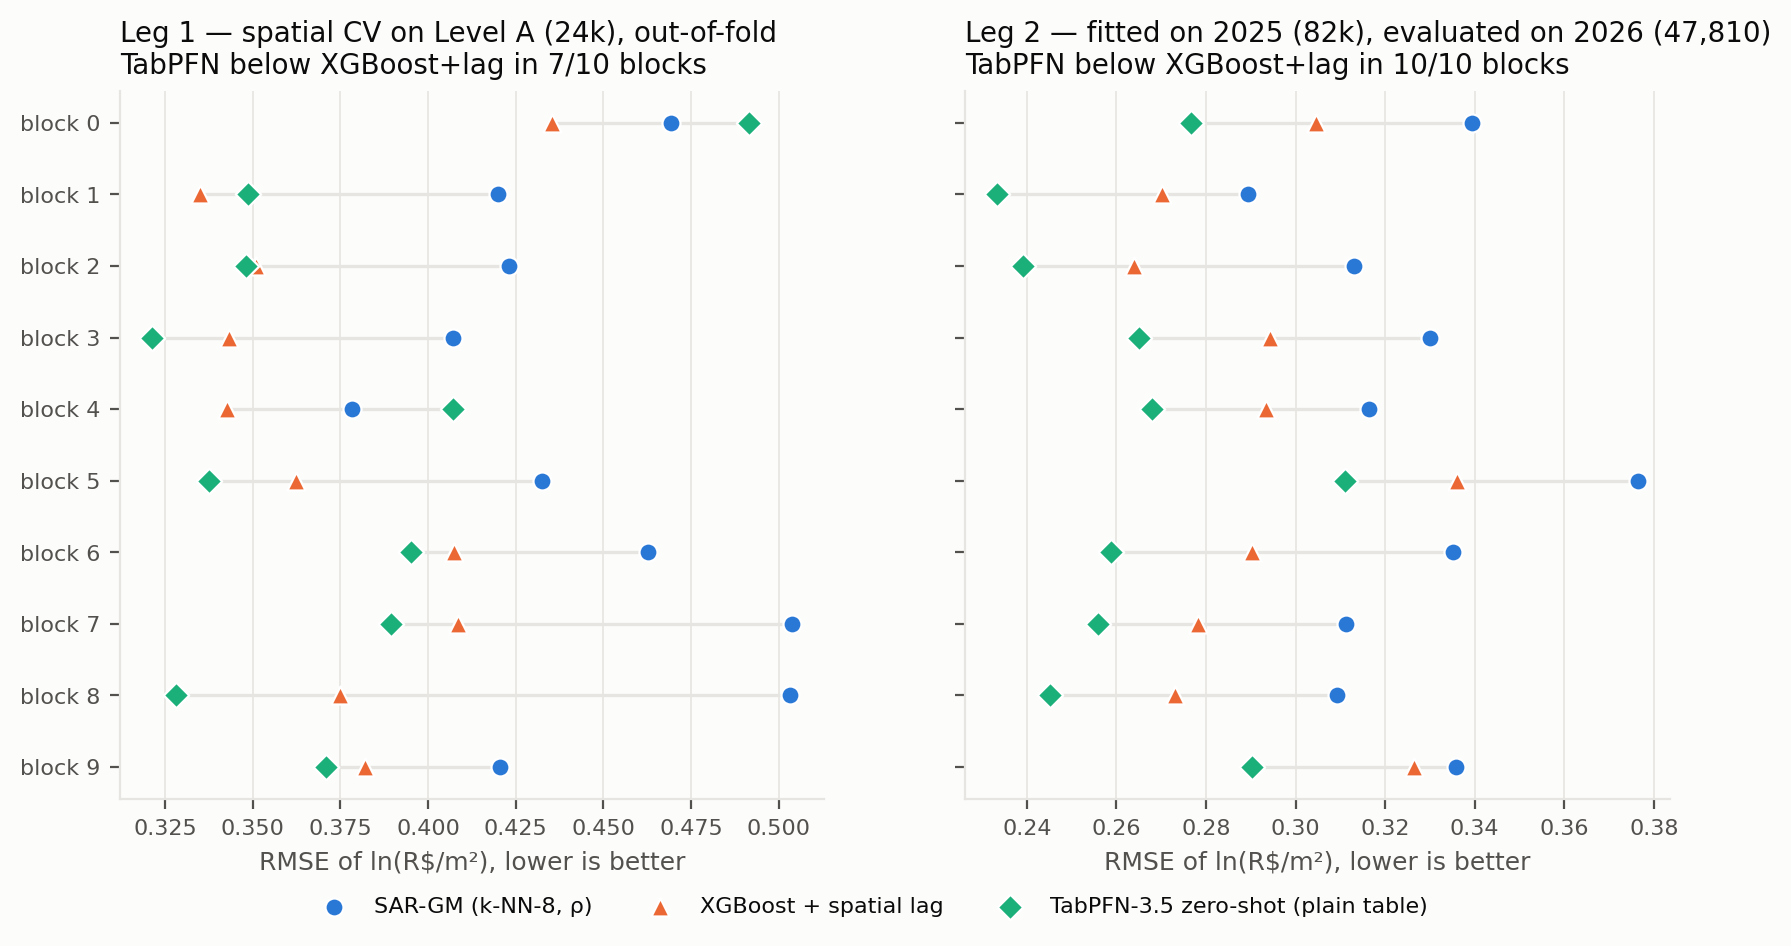
\includegraphics[width=\textwidth]{fig2_per_block_rmse.png}
\caption{RMSE per block, both legs.}
\end{subfigure}\hfill
\begin{subfigure}[t]{0.49\textwidth}
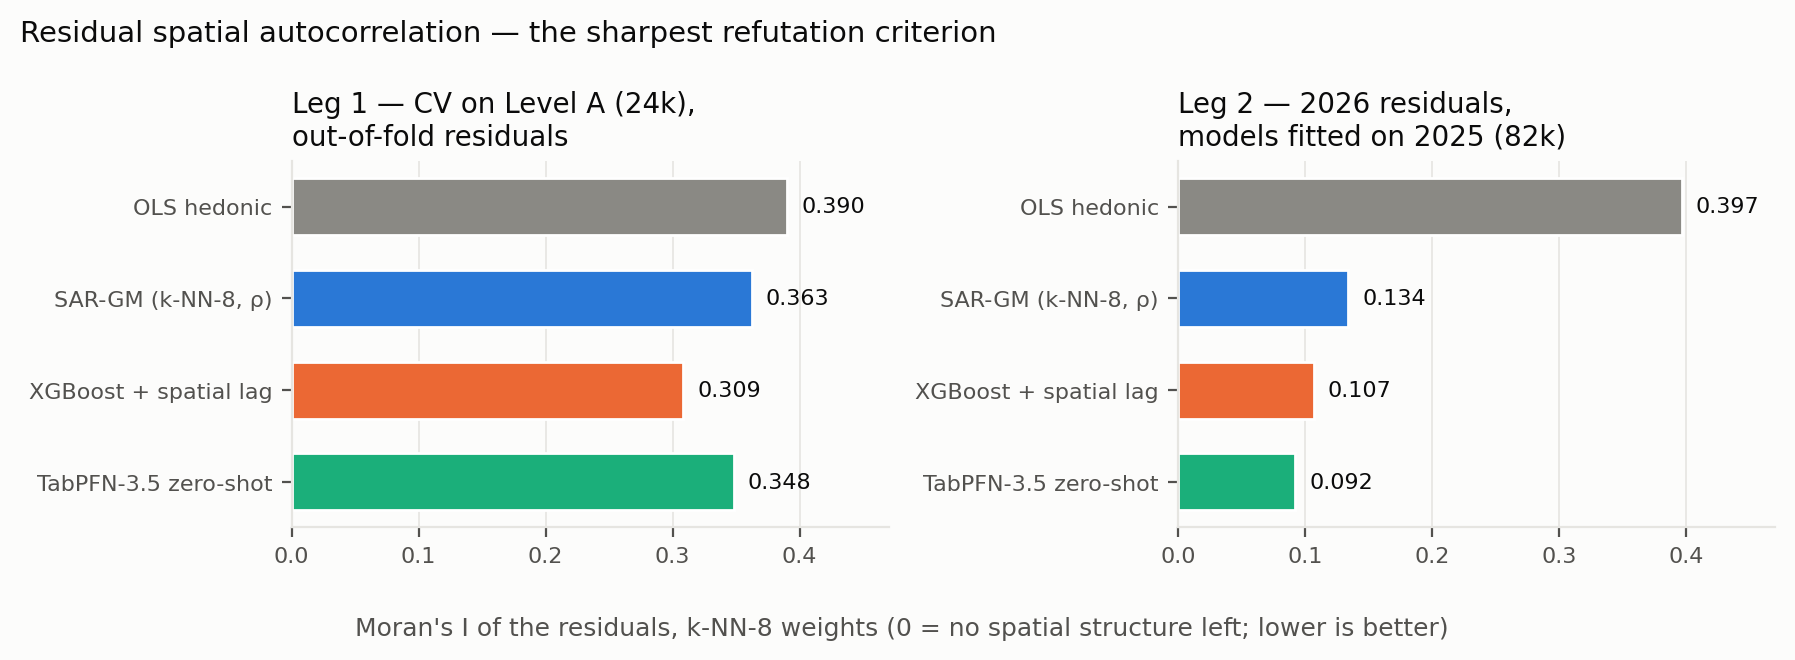
\includegraphics[width=\textwidth]{fig5_moran.png}
\caption{Residual Moran's $I$, both legs.}
\end{subfigure}
\caption{Left of each panel: leave-one-block-out CV on Level A; right: 2026 out-of-time, full
2025 base. \todo{Check panel layout against the actual figures and adjust the caption.}}
\label{fig:blocks-moran}
\end{figure}

\begin{figure}[t]
\centering
\begin{subfigure}[t]{0.55\textwidth}
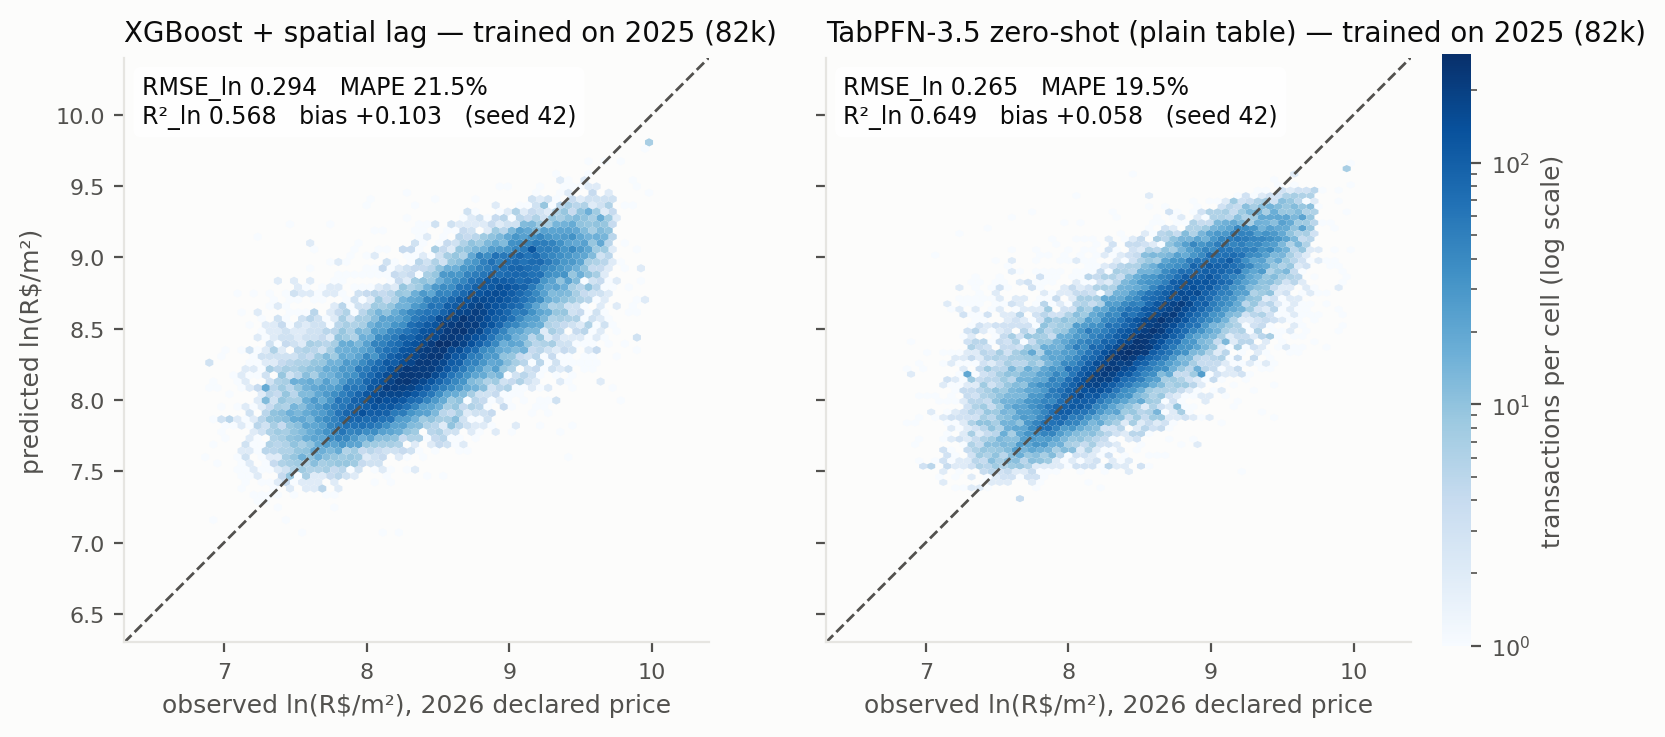
\includegraphics[width=\textwidth]{fig3_pred_vs_obs_2026.png}
\caption{Predicted vs observed, 2026.}
\end{subfigure}\hfill
\begin{subfigure}[t]{0.43\textwidth}
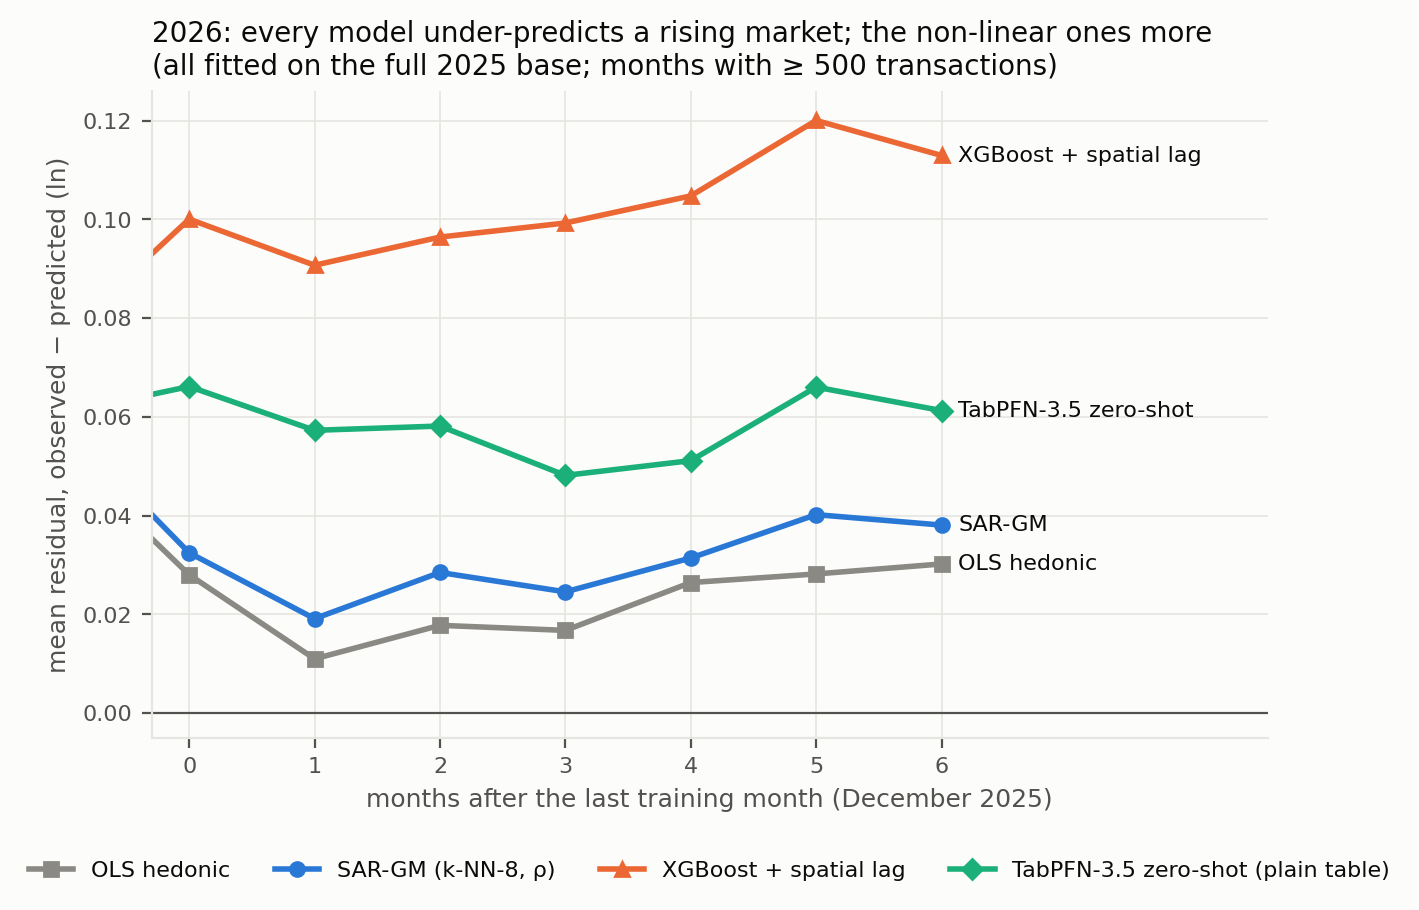
\includegraphics[width=\textwidth]{fig4_months_ahead_bias.png}
\caption{Mean residual by month ahead.}
\end{subfigure}
\caption{The rising market of 2026: every model under-predicts, the non-linear learners more so.}
\label{fig:bias}
\end{figure}

\subsection{Robustness: financed transactions only}
\label{sec:robust}

\begin{table}[h]
\centering\small
\caption{Both legs on financed deals only: 7{,}211 Level A rows (CV) and the same rows fitted once
and scored on the 20{,}052 financed transactions of 2026.}
\label{tab:fin}
\begin{tabular}{lcccccc}
\toprule
Model & CV RMSE & CV MAPE & CV $I$ & 2026 RMSE & 2026 MAPE & 2026 $I$ \\
\midrule
OLS hedonic & 0.354 & 28.5\% & 0.343 & 0.343 & 26.5\% & 0.491 \\
SAR lag & 0.344 & 28.1\% & 0.342 & 0.286 & 22.0\% & 0.297 \\
XGBoost + lag & 0.286 & 23.0\% & 0.327 & 0.221 & 16.7\% & 0.160 \\
TabPFN-3.5, zero-shot & \textbf{0.269} & \textbf{21.1\%} & \textbf{0.279} & \textbf{0.207} & \textbf{15.3\%} & \textbf{0.143} \\
\bottomrule
\end{tabular}
\end{table}

Cleaner prices lower every error and leave the ranking unchanged. The plain-table model now beats
XGBoost+lag in the block CV as well ($\Delta$RMSE $= -0.017$ $[-0.032, -0.003]$, $p = 0.049$, 8 of
10 blocks) and the partial refutation on the residual criterion does not reappear: it leaves less
spatial structure than the spatial XGBoost in both legs. The headline results do not depend on the
cash deals retained by the under-declaration filter.

\subsection{Explaining an estimate}

\begin{figure}[t]
\centering
\begin{subfigure}[t]{0.49\textwidth}
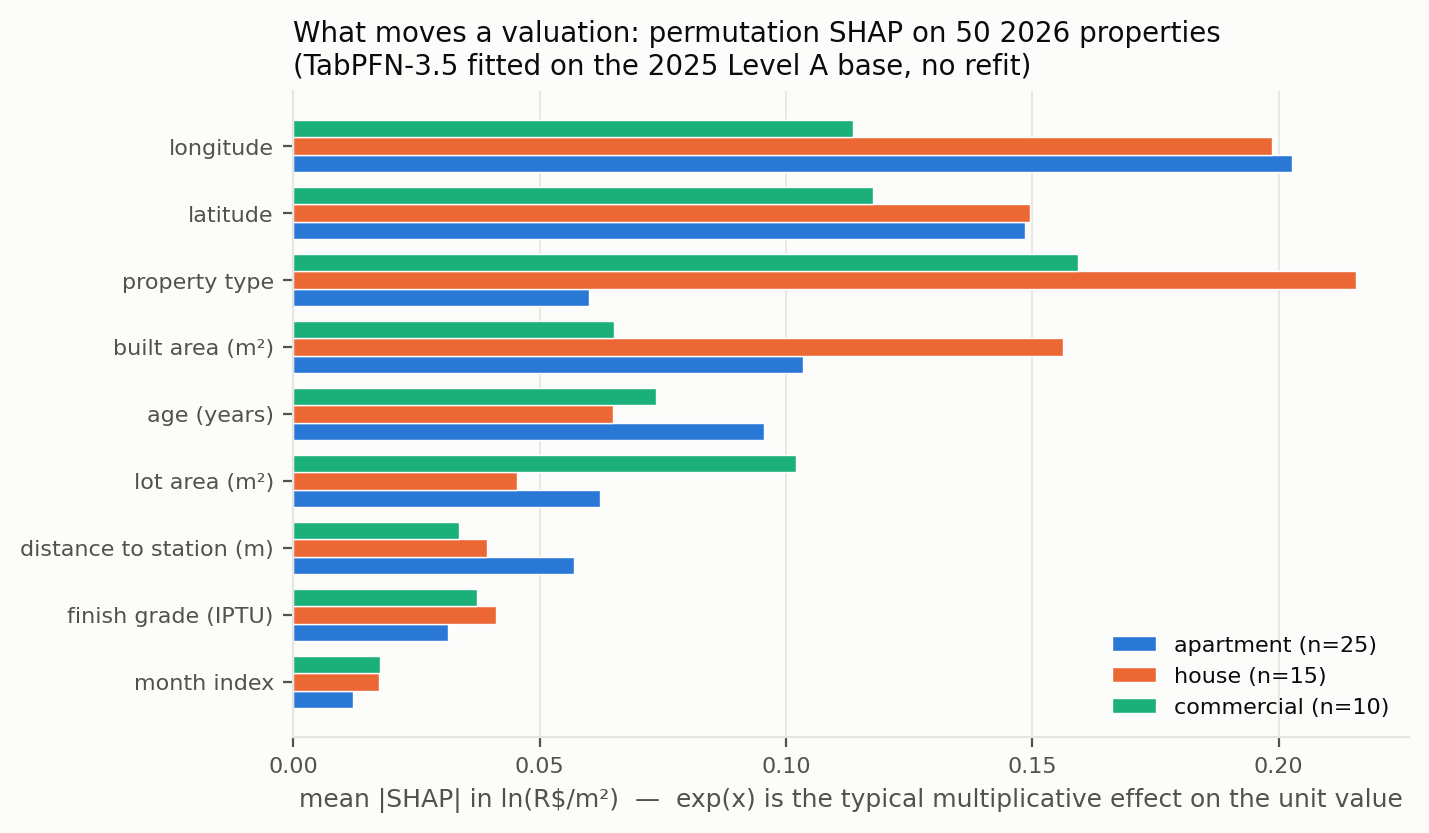
\includegraphics[width=\textwidth]{fig6_shap_importance.png}
\caption{Mean $|$SHAP$|$ by feature and type.}
\end{subfigure}\hfill
\begin{subfigure}[t]{0.49\textwidth}
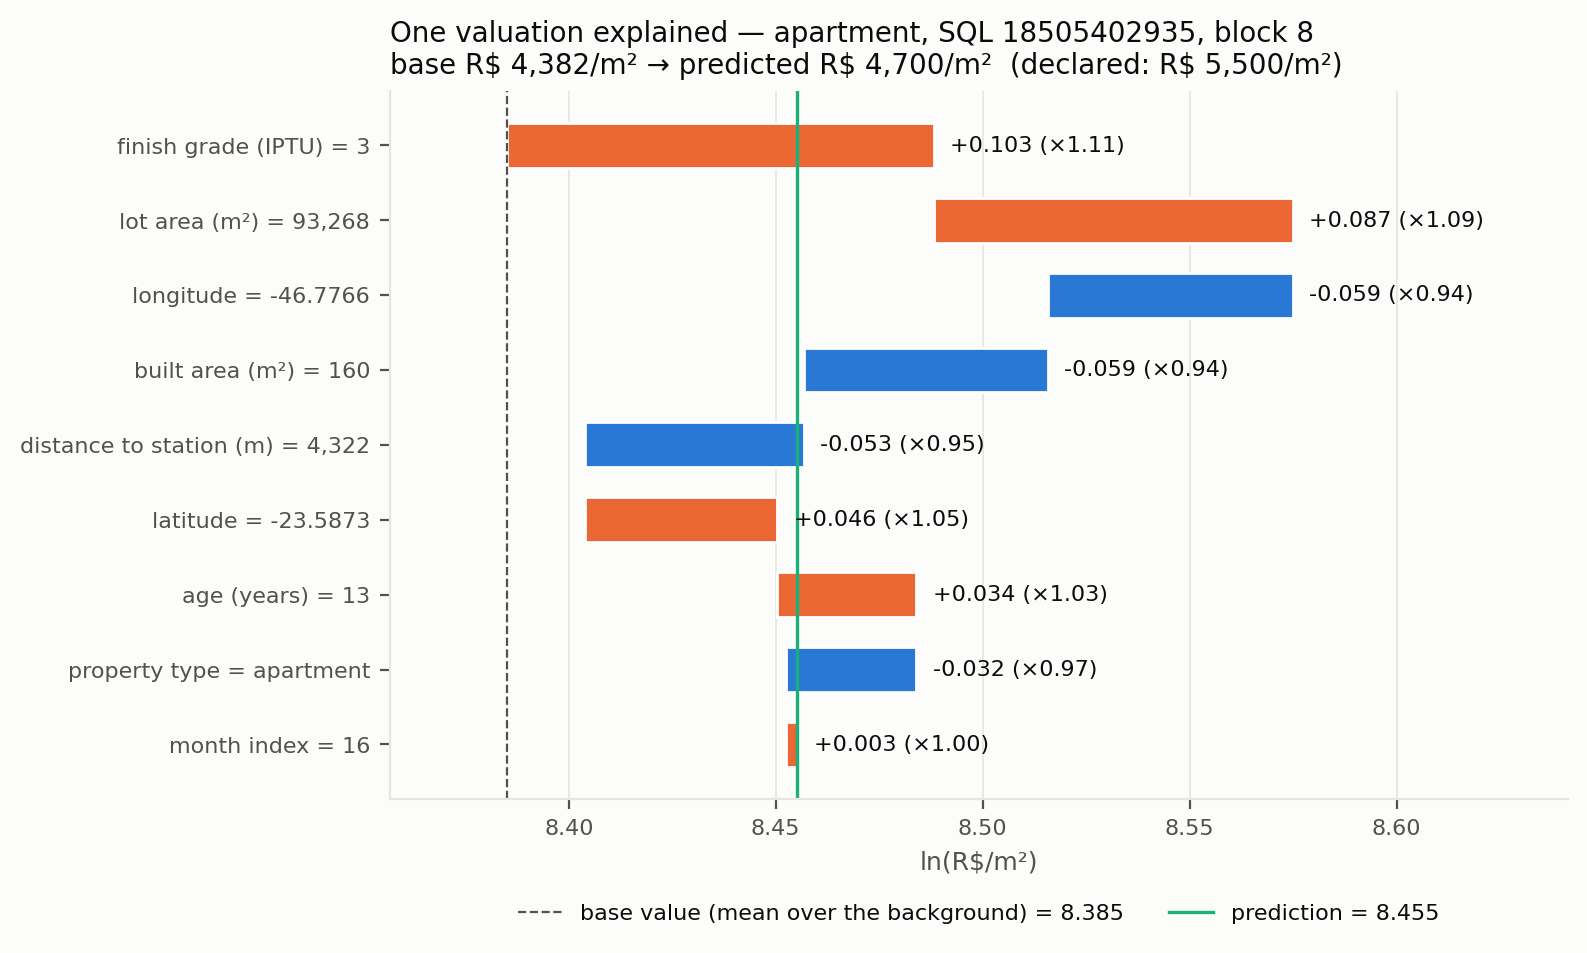
\includegraphics[width=\textwidth]{fig8_shap_waterfall.png}
\caption{One valuation, base value to estimate.}
\end{subfigure}
\caption{Permutation SHAP on 50 transactions of 2026 (independent masker, 20-row background), model
reloaded from its cached record. Values in log units; $e^{\text{SHAP}}$ is the multiplier on the
unit value.}
\label{fig:shap}
\end{figure}

Permutation SHAP \citep{lundberg2017shap} on 50 stratified 2026 transactions the model had never
seen ranks longitude (mean $|$SHAP$|$ 0.184, a typical $\times 1.20$ on the unit value) and latitude
(0.143, $\times 1.15$) as the two strongest inputs, ahead of property type (0.127), built area
(0.112) and age (0.082). Directions match appraisal experience: age and distance to a station pull
the unit value down, finish grade pushes it up, larger built areas lower the price per square metre.
The two raw coordinates carry, inside the model, the signal the baselines encode with a weights
matrix. \todo{One sentence on the reconstructed-prediction check (RMSE 0.296 on the sample).}

\section{Discussion}
\label{sec:discussion}

\todo{Four paragraphs. (1) Reading the two legs together: extrapolation to unseen blocks is where
explicit spatial modelling still earns its keep on the residual criterion, while inside the city
one year ahead the plain table wins outright; discuss why (in-context learning over 24--82k rows
recovers neighbourhood structure from the coordinates when neighbours exist in context). (2) The
trend bias: none of the non-linear models extrapolates the month index; what appraisal practice
would do (index adjustment) and why it was not applied here. (3) Cost and engineering: seconds
against nested tuning and weights matrices; what this means for mass appraisal at municipal scale
and for the Brazilian standard NBR 14653-2 (the standard's precision grades need intervals, which
the model provides as predictive quantiles --- future work). (4) Limitations: centroid coordinates,
declared prices, one city, hosted model (no access to internals, hence no per-row attribution for
the regression head), no comparables from inside the model.}

\section{Conclusion}
\label{sec:conclusion}

\todo{One paragraph restating the hypothesis, the verdict per leg, and what would change the
verdict (another city, listings vs declared prices, a model with row-level attribution).}

\section*{Reproducibility}
Code, cleaned data, cached model responses and every number in this paper are at
\url{https://github.com/abenvenho/tabpfn-itbi-sp} (Apache-2.0). The pipeline was re-run from a
clean clone; the three bases were rebuilt byte-identical from the raw public workbooks.

\section*{Acknowledgements}
\todo{Prior Labs hackathon; AI assistance statement (code developed with Claude; methodological
decisions by the author).}

\bibliographystyle{plainnat}
\bibliography{refs}

\appendix
\section{Filter chain}
\label{app:filters}
\todo{Table with the per-step record counts from \texttt{data/filter\_report.md}.}

\section{Geographically weighted XGBoost: feasibility pilot}
\label{app:gxgb}
\todo{Two sentences and the timing numbers from \texttt{results/gxgb\_timing\_pilot.json}.}

\section{Hyper-parameters}
\label{app:hparams}
\todo{XGBoost search space and the selected values per fold (\texttt{results/xgb\_params\_*.json});
TabPFN-3.5 settings (version, thinking effort, timeout).}

\end{document}
